\documentclass[a4paper,twoside]{article}

\usepackage{epsfig}
\usepackage{subfigure}
\usepackage{calc}
\usepackage{amssymb}
\usepackage{amstext}
\usepackage{amsmath}
\usepackage{amsthm}
\usepackage{multicol}
\usepackage{pslatex}
\usepackage{apalike}
\usepackage{SCITEPRESS}     % Please add other packages that you may need BEFORE the SCITEPRESS.sty package.
\usepackage[hyphens]{url}

\subfigtopskip=0pt
\subfigcapskip=0pt
\subfigbottomskip=0pt

% image shadow 
\usepackage{tikz}
\usetikzlibrary{shadows,calc}

% some parameters for customization
\def\shadowshift{3pt,-3pt}
\def\shadowradius{6pt}

\colorlet{innercolor}{black!60}
\colorlet{outercolor}{gray!05}

% this draws a shadow under a rectangle node
\newcommand\drawshadow[1]{
    \begin{pgfonlayer}{shadow}
        \shade[outercolor,inner color=innercolor,outer color=outercolor] ($(#1.south west)+(\shadowshift)+(\shadowradius/2,\shadowradius/2)$) circle (\shadowradius);
        \shade[outercolor,inner color=innercolor,outer color=outercolor] ($(#1.north west)+(\shadowshift)+(\shadowradius/2,-\shadowradius/2)$) circle (\shadowradius);
        \shade[outercolor,inner color=innercolor,outer color=outercolor] ($(#1.south east)+(\shadowshift)+(-\shadowradius/2,\shadowradius/2)$) circle (\shadowradius);
        \shade[outercolor,inner color=innercolor,outer color=outercolor] ($(#1.north east)+(\shadowshift)+(-\shadowradius/2,-\shadowradius/2)$) circle (\shadowradius);
        \shade[top color=innercolor,bottom color=outercolor] ($(#1.south west)+(\shadowshift)+(\shadowradius/2,-\shadowradius/2)$) rectangle ($(#1.south east)+(\shadowshift)+(-\shadowradius/2,\shadowradius/2)$);
        \shade[left color=innercolor,right color=outercolor] ($(#1.south east)+(\shadowshift)+(-\shadowradius/2,\shadowradius/2)$) rectangle ($(#1.north east)+(\shadowshift)+(\shadowradius/2,-\shadowradius/2)$);
        \shade[bottom color=innercolor,top color=outercolor] ($(#1.north west)+(\shadowshift)+(\shadowradius/2,-\shadowradius/2)$) rectangle ($(#1.north east)+(\shadowshift)+(-\shadowradius/2,\shadowradius/2)$);
        \shade[outercolor,right color=innercolor,left color=outercolor] ($(#1.south west)+(\shadowshift)+(-\shadowradius/2,\shadowradius/2)$) rectangle ($(#1.north west)+(\shadowshift)+(\shadowradius/2,-\shadowradius/2)$);
        \filldraw ($(#1.south west)+(\shadowshift)+(\shadowradius/2,\shadowradius/2)$) rectangle ($(#1.north east)+(\shadowshift)-(\shadowradius/2,\shadowradius/2)$);
    \end{pgfonlayer}
}

% create a shadow layer, so that we don't need to worry about overdrawing other things
\pgfdeclarelayer{shadow} 
\pgfsetlayers{shadow,main}

\newsavebox\mybox
\newlength\mylen

\newcommand\shadowimage[2][]{%
\setbox0=\hbox{\includegraphics[#1]{#2}}
\setlength\mylen{\wd0}
\ifnum\mylen<\ht0
\setlength\mylen{\ht0}
\fi
\divide \mylen by 120
\def\shadowshift{\mylen,-\mylen}
\def\shadowradius{\the\dimexpr\mylen+\mylen+\mylen\relax}
\begin{tikzpicture}
\node[anchor=south west,inner sep=0] (image) at (0,0) {\includegraphics[#1]{#2}};
\drawshadow{image}
\end{tikzpicture}}
% end image shadow 

\begin{document}

\title{YouPower --  A Social App for User Engagement in Power Grids
%\subtitle{Preparation of Camera-Ready Contributions to SCITEPRESS Proceedings} 
}

\author{\authorname{First Author Name\sup{1}, Second Author Name\sup{1} and Third Author Name\sup{2}}
\affiliation{\sup{1}Institute of Problem Solving, XYZ University, My Street, MyTown, MyCountry}
\affiliation{\sup{2}Department of Computing, Main University, MySecondTown, MyCountry}
\email{\{f\_author, s\_author\}@ips.xyz.edu, t\_author@dc.mu.edu}
}

\keywords{Power Grid, Smart Grid, Energy Community, Social Participation, Social App, YouPower, Prosumer}

\abstract{The abstract should summarize the contents of the paper and should contain at least 70 and at most 200 words. The text must be set to 9-point font size. \vspace*{2cm}}

\onecolumn \maketitle \normalsize \vfill

\section{\uppercase{Introduction}}
\label{sec:introduction}

\noindent 
\textit{YouPower} is an open source platform designed to explore the potential and challenges of supporting social participation, awareness and engagement of smart gird users for energy conservation and load shifting\footnote{\url{http://www.civisproject.eu}, \url{https://app.civisproject.eu}.}. Combining smart sensing and web technologies among others,
YouPower features a social smart grid application (developed as a hybrid mobile app) that can connect users to friends, families and local communities to learn and take energy actions that are relevant to them together. The app encourages an energy-friendly lifestyle and can be linked to users' energy consumption and production data for quasi real-time and historical prosumption information. 
% 
The goal of the project is to make energy more visible, to promote environmental and social values, to inform users' know-how about sustainable consumption, and to facilitate users to take energy conservation and load shifting actions in their everyday life together with local communities \cite{Huang2014,Huang2015c,Huang2016}. 
%  

Research topics related to merging the strength of Social Networks (SNs) with that of smart grid applications have caught much attention recent years following the success of several popular SN platforms \cite{Boslet2010,Chima2011,Erickson2012,Fang2013,Huang2015}. 
% 
Some conducted surveys to understand user needs for energy services combining SNs \cite{Silva2012}. Some studied connecting smart meters (or smart homes) as SNs for
energy management and sharing \cite{Ciuciu2012,Steinheimer2012}. 
Simulation models are developed to study demand side management %and value-added web services 
taking into consideration SN aspects \cite{De-Haan2011,Lei2012,Chatzidimitriou2013} and to demonstrate the feasibility of
coordination in load balancing \cite{Worm2013,Skopik2014}. There are also works that visualize smart meter and appliance-level consumption data, and provide comparative feedback among households\cite{Petkov2011,Weiss2012,Dillahunt2014}.
% 
Our research interest expands on the related work, and places an emphasis on smart grid user communities and collective actions. 

The research is performed within the framework of the EU FP7 CIVIS project. It has test sites in Stockholm (Sweden) and Trento (Italy) with domestic energy consumers. 
% 
In Sweden, those who buy a home officially own the right to inhabit the estate and must join a corresponding \textit{housing cooperative} 
that owns and maintains its estates. The test site in Stockholm is composed of \textbf{sixteen(?)} housing cooperatives, each of which has annually elected board members who make energy related decisions on behalf of the cooperative members. 
In the case of Trento test site, two local \textit{electricity consortia} produce and sell renewable (hydro and solar) energy to consortium members. Household rooftop PV panels are also common in this region.  The consortia are highly interested in load shifting to optimize the use of local renewables reducing dependency on the national supply. 
These two types of communities are at the center of YouPower design. 
% 
The rest of this paper presents the design process of YouPower, gives an overview of the platform, and discuss in more detail its design concept.



\begin{figure*}[t!]
\begin{center}\footnotesize
	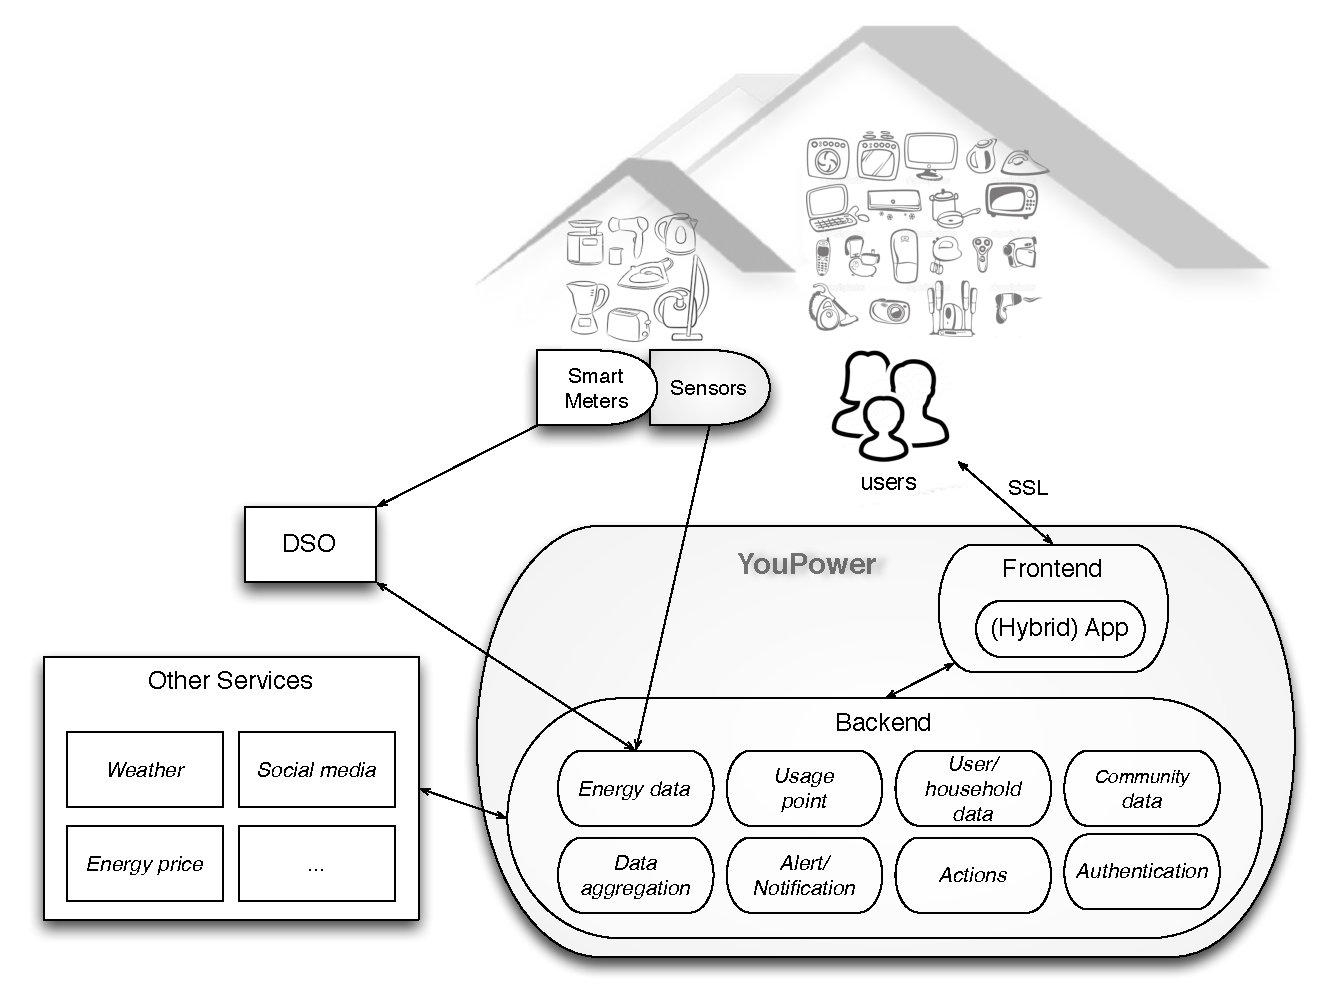
\includegraphics[width=.7\textwidth]{img/civis_platform_overview.pdf}\\
	DSO (Distribution System Operators),  SSL (Secure Sockets Layer)
	\caption{YouPower system overview}\label{fig:platform}
\end{center}
\end{figure*}

\section{\uppercase{State of the Art}}

\noindent Prior to designing YouPower, we first review existing proposals for social platforms in the context of power grids. Second, we summarize the findings about success of different consumer behavior change interventions and strategies. One of the repeatedly reported drawbacks of different solutions aiming to involve consumers is a lack of their sustained use \cite{edward2015review}. Iterative and lean design process that we adopt is suggested as a promising approach to tackle this problem \cite{schwartz2014people}.

Weiss et al.~\cite{weiss2012powerpedia} developed a smartphone community platform, PowerPedia. The platform works in connection with smart meters and enables users to identify and upload their own appliance-level consumption statistics. After upload, the users can compare their appliance consumption with other users. The platform was evaluated in a lab setting and the test users rated favorably social comparison features and appliance level statistics.

Community Monitor \cite{dillahunt2014understanding} is a social energy app deployed on tablets that was tested in two distinct communities for 4-10 months. The app featured leaderboard, message board and shared actions ("ways to save"). The findings from the trial revealed importance of environmental, social and cultural context for the app use. For instance, the existence of common spaces for community members to interact and knowledge of other users supported the app use. On the other hand, shorter length of residence or rented apartment negatively affected the engagement. Community Monitor did not manage to engage users around the message board feature.

Petkov et al.~\cite{petkov2011motivating} delve more into the details of comparative feedback. Their findings confirm importance of comparisons to similar users in terms of energy consumption and neighbors. However, if the competition features are included, then the users preferred to compete with the people whom they actually know and especially with their friends. 

X Considering the analytical frames and the CIVIS use cases, we chose a set of platform features and translated those into three self-contained and composable parts to be included in the CIVIS (front-end) application (hereinafter abbreviated as CIVIS app): 
%\begin{enumerate}
%\item \nameref{sect:tips}
%\item \nameref{sect:brf}
%\item \nameref{sect:load_shifting}
%\end{enumerate}



With peer review results and users' feedback on the design, adaptations and changes are made to suit user needs and to achieve the CIVIS research goal. 
In general, the application aims to enhance users' energy know-how through action suggestions that are implementable in everyday life, engage users in energy communities with understandable and actionable information and feedback, and facilitate community interaction and self-teaching by means of group discussions.
%

Given the time and resource constraints, the app can not be developed all-in-one cross-platform (for phones, tablets and computers). We chose to design the front-end as a mobile app. This means that the app design has layouts and user interactions that suit (small) phone screens. %The consideration is multi-fold. 
Western Europe has a large mobile phone internet user base\footnote{
Between 2013 and 2017, the penetration rate of mobile phone internet users among mobile phone users will rise from 49.0\% to 77.8\%. See more at:\url{ http://www.emarketer.com/Article/Nearly-Half-of-Western-Europeans-Will-Use-Mobile-Web-This-Year/1010510\#sthash.AaVfsqIU.dpuf}}. Many surveys show that mobile apps have advantages such as creating deeper user engagement, easy sharing, among others\footnote{\url{https://infomedia.com/blog/the-advantages-of-mobile-apps/}, \url{https://econsultancy.com/blog/62326-85-of-consumers-favour-apps-over-mobile-websites/}}. This makes mobile app a good choice given the goal of the CIVIS platform. Once developed, mobile apps can also be more easily transformed to web browser versions, while the reverse is more difficult. The back-end of the CIVIS platform will remain mostly the same independent of the front-end alternatives. 


\section{\uppercase{YouPower Overview}}
\label{sect:overview}

\noindent Figure~\ref{fig:platform} gives an overview of the CIVIS YouPower platform. 
It is composed of (I) the \textit{energy sensor level services} mainly dealing with energy data collection; and (II) the \textit{energy data level and social level services} mainly dealing with energy data analytics as well as user, household and community management among others. 

\begin{figure}[h!]
\begin{center}\footnotesize
	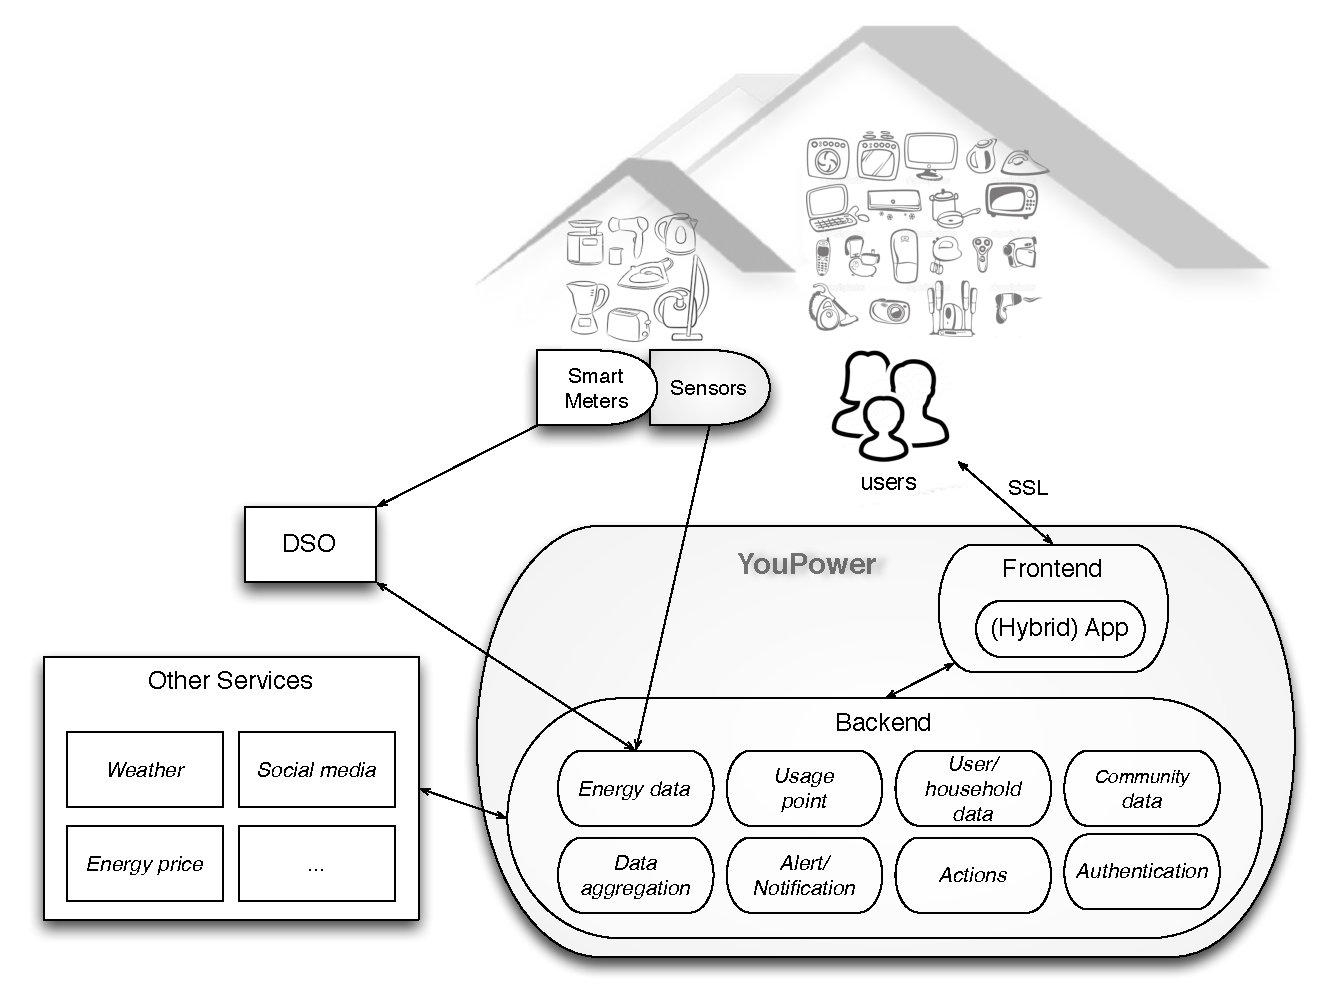
\includegraphics[width=1.0\linewidth]{img/civis_platform_overview.pdf}\\
	DSO (Distribution System Operators),  SSL (Secure Sockets Layer)
	\caption{YouPower Platform Overview}\label{fig:platform}
\end{center}
\end{figure}

(I) \textit{Energy sensor level services:} CIVIS project installed hardware (smart plugs and sensors) and software required for appliance-level energy data collection. The hardware/software choices differ in the two sites due to local circumstances. For example, \textit{Smappee} for 40 households in Stockholm, and \textit{CurrentCost} for 79 households in Trento\footnote{All trademarks used in this paper are properties of their respective owners. The use of any trademark does not vest in the authors any trademark ownership rights in such trademarks, nor does the use of such trademarks imply any affiliation with or endorsement of the authors by such owners.}. Trento also installed Amperometric clamps for PV prodcution measures.
Household-level energy data is measured by smart meters and provided by local DSOs (Distribution System Operators). 

(II) \textit{Energy data level and social level services:} These services are provided by the YouPower app and its back-end. The design of the YouPower app (and its back-end) consists of three self-contained composable parts: (A) \textit{House Cooperatives} (contextualized and deployed to the Stockholm test site); (B) \textit{Demand-Side Management} (contextualized and deployed
to the Trento test site); and (C) \textit{Action Suggestions} (contextualized and deployed to both test sites). They are discussed in Section~\ref{sect:design_concept}.

\section{\uppercase{Design Concept}}
\label{sect:design_concept}

\noindent Given time and resource constraints, the YouPower app can not be developed all-in-one cross-platform (for phones, tablets and computers). We chose to design the front-end as a hybrid mobile phone app, i.e. its UI design has layouts that suit phone screens, %The consideration is multi-fold. 
%Western Europe has a large mobile phone internet user base\footnote{Between 2013 and 2017, the penetration rate of mobile phone internet users among mobile phone users will rise from 49.0\% to 77.8\%. See more at: \url{ http://www.emarketer.com/Article/Nearly-Half-of-Western-Europeans-Will-Use-Mobile-Web-This-Year/1010510\#sthash.AaVfsqIU.dpuf}}. Many surveys show that mobile apps have advantages such as creating deeper user engagement, easy sharing, among others\footnote{\url{https://infomedia.com/blog/the-advantages-of-mobile-apps/}, \url{https://econsultancy.com/blog/62326-85-of-consumers-favour-apps-over-mobile-websites/}}. This makes mobile app a good choice given the goal of the CIVIS platform. 
since mobile apps can be more easily transformed to web browser versions, while the reverse is more difficult. The back-end of the YouPower platform will remain mostly the same independent of the front-end alternatives. 

\subsection{Housing Cooperatives}
\label{sect:brf}

This part of the YouPower app is designed for the community of housing cooperatives (\textit{Bostadsr{\"a}ttsf{\"o}rening} or \textit{Brf} in Swedish) in the Stockholm test site \cite{Hasselqvist2016}.
Similar housing ownership and management models exist in a number of EU and non-EU countries, which allow potential wider application of the design.
A housing cooperative annually elects a board which manages cooperative properties and decides on energy contracts, maintains energy systems, and proposes investments in energy efficient technologies. Since board members are volunteers who may have limited knowledge of energy or building management, this part of the app aims to support board members in energy management, in particular energy reduction actions. Cooperative members can also use the app to follow energy decisions and works of the cooperative. Additionally, the app can be of interest by building management companies working with housing cooperatives. 
The information presented in the app is visible for these user
groups and shared between housing cooperatives. This openness of energy data is key to
facilitating  users in sharing experiences relevant for taking energy reduction actions.

\subsubsection{Linking energy data to energy reduction actions}

The design links energy data with energy reduction actions taken (Figure~\ref{fig:Figure201_Actions}), both at cooperative levels, making the impact of energy actions visible to users. The energy use is divided into heating \& hot water (from district heating), and facilities electricity (in apartment buildings). Users can switch between the views per month or per year to show overall changes. %Since the energy data is shared between cooperatives there may also be privacy concerns related to opening up data of higher granularity to people outside of the own cooperative. 
%
\begin{figure}[h!]
	\centering
	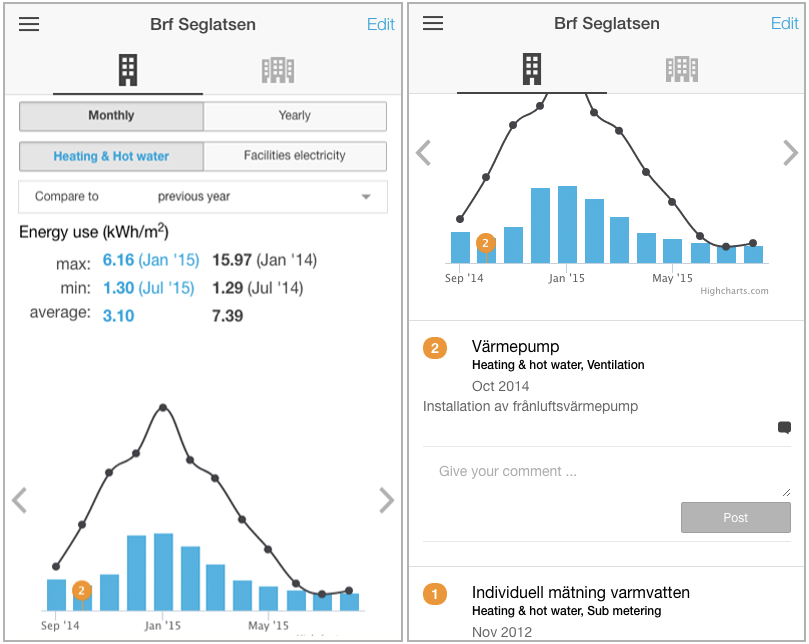
\includegraphics[width=1\linewidth]{img/Figure201_Actions.png}
	\caption{Heasting \& hot water use graph. Blue bars show the current year's use per month; the black line shows that of previous year. Energy reduction actions taken are mapped to the time of action and listed below.}
	\label{fig:Figure201_Actions}
\end{figure}
%
Users with editing rights, typically board members, can  add energy reduction actions that the cooperative has taken, e.g., improvement of ventilation, lighting or heating systems, 
and the related cost.
Trusted energy or building management companies can also get editing rights to add energy reduction actions they took on behalf of the cooperative. 
Added actions appear at the month when each action was taken and are listed below the graph. When clicking on an action in the list, the details of the action are shown.
% 
To make the impact of actions visible, users can compare the energy use of the viewed months to that of a previous year. This can be used e.g. by a cooperative to explore what energy reduction actions to take in the future by learning actions taken by other cooperatives and what the effects were in relation to costs.

\subsubsection{Comparing housing cooperatives}

\begin{figure}
	\centering
	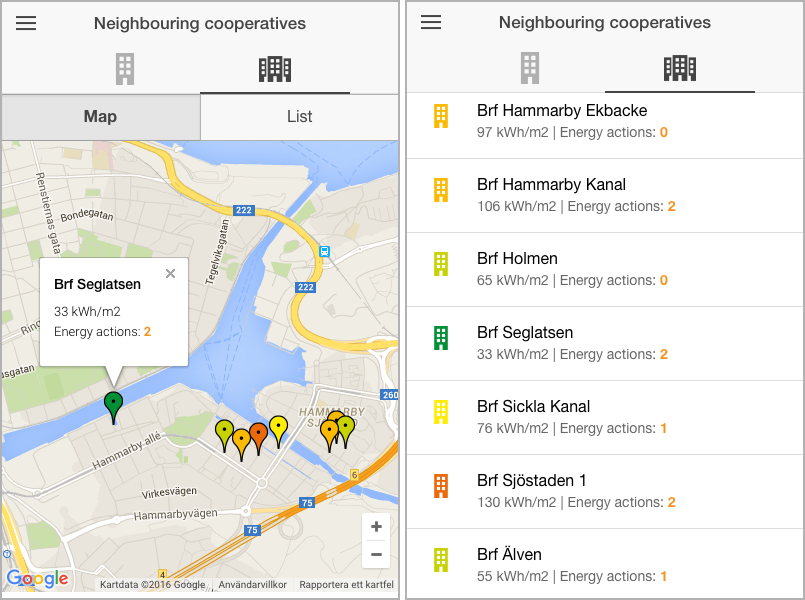
\includegraphics[width=0.99\linewidth]{img/Figure202_Housing_cooperatives_comparison.png}
	\caption{Map and list view of participating housing cooperatives. The energy performance of cooperatives is indicated by colour and in numbers.}
	\label{fig:Figure202_Housing_cooperatives_comparison}
\end{figure}

The cooperatives that are registered for the app are displayed in a map or list view (Figure~\ref{fig:Figure202_Housing_cooperatives_comparison}). Their icons are color coded (from red to green) based on each cooperative's energy performance, i.e. from high to low energy use per heated area, scaled according to the Swedish energy declaration for buildings\footnote{\url{http://www.boverket.se/sv/byggande/energideklaration/energideklarationens-innehall-och-sammanfattning/sammanfattningen-med-energiklasser/energiklasser-fran-ag/}}. 
%  but it is calibrated to only include measured energy use for heating and hot water, which is the greatest part of the energy use. In the Swedish energy declarations, facilities electricity is also added but that often requires estimations of different factors to make the number comparable.
% 
Users can also see the energy performance as a number (in kWh/m$^2$), and the information about energy reduction actions of the cooperatives. %The number of actions is important to display to make energy reduction efforts of housing cooperatives with a high energy performance (e.g. due to poor construction of the building) visible. 
% 
During stakeholder studies, energy managers in cooperative boards stressed the importance of knowing the difference between cooperatives in order to understand the difference in their energy performance. Thus, the design also includes information about cooperatives (Figure~\ref{fig:Figure204_Neighbourhood_average}) such as the number of apartments and heated areas in a cooperative, a building's construction year, and types of ventilations (e.g. with or without heat recovery).
% 
Users can compare a cooperative's energy use per month or per year to another cooperative or to the neighborhood average. The electricity use is also displayed per area (kWh/m$^2$) to make it comparable.
\begin{figure}
\centering
\shadowimage[width=.55\linewidth]{img/brf.pdf}
\caption{Facilities electricity use graph. Information about housing cooperatives and actions is displayed at the top. Green bars show the housing cooperative's current year's use per month; the black line shows the average use of all housing cooperatives}
\label{fig:Figure204_Neighbourhood_average} 
\end{figure}

\subsubsection{Sharing experiences}

% The details about each energy action taken by a cooperative, together with the effects on the energy use, provides information that could support other cooperatives in learning more about which energy reduction actions are effective. 
% In addition to the aforementioned information, 
A cooperative interested in taking an action may wish to know more, e.g. which contractor was chosen for an investment and why or how to get buy-in from cooperative members. The design provides commenting functions for each action added, where users can post questions and exchange experiences. The cooperatives can also add email addresses of their contact persons, which are visible on each cooperative's app page.
% 
Sharing experiences certainly also happens outside of the digital world, e.g. during meetings of cooperative boards or with local energy networks. The app aims  to support discussions and knowledge exchange also in such situations, where someone can easily demonstrate the impact of an energy investment with smart phones.

%Three main categories of features are designed for this part of YouPower: energy information about a user's own housing cooperative, energy information about other housing cooperatives, and support for communication between energy managers.
%Expected primary users are energy managers and board members of housing cooperatives. Secondary users are ordinary cooperative members. 
%
%Housing cooperative energy information includes comparative energy performance %(kWh /m$^{2}$)\footnote{We chose to use kWh in this case since cooperative managers have fairly good knowledge of energy units and the visualization is comparative.} 
%and the cooperative's monthly and yearly energy use, divided into heating (including hot water) and facilities electricity. Energy actions that have been taken are listed in relation with energy consumptions. 
%A user can see when different actions, such as energy information, optimisation or investments, were previously taken and see more details about the actions. By comparing the energy use with previous periods, the user can also see the impact of the actions.
%% 
%In the same way that the users can view information about their own cooperatives, they can also see the energy performance and energy actions taken by other cooperatives. This allows energy managers and others who are interested to e.g. explore the effect of a neighbouring cooperative's actions on their energy use and read about how they carried out an investment and which contractor was used. 
%% 
%To further support collaboration and knowledge exchange between housing cooperatives, there is a discussion group dedicated for energy managers. Within the group they have the possibility of creating discussion topics of their interests. In this way, the discussion of the occasional meetings with the local energy network can be extended to continue online.

%\subsubsection{Design Evaluation}
%
%The design was evaluated with three energy managers and the feedback was incorporated in the design improvement of the application. The energy managers would primarily want to use the app to find housing cooperatives with similar challenges and see what actions they had taken. They also thought the app would be helpful for deciding which companies can be trusted based on what other housing cooperatives had done and what the effects were on the energy use. The energy managers doubted that other members in their cooperatives would be very interested in following the cooperative's energy use, but they thought the app might be useful for engaging members in specific questions. 

% % % ITALIAN TEST SITE

\subsection{Demand-Side Management} 
\label{sect:load_shifting}

This part of the YouPower app is designed for the Trento test site and can have wider application.
It provides users historical and quasi real-time consumption and production information, and facilitates users to leverage load elasticity in order to maximize self-consumption of rooftop PV productions. 
Energy data is displayed at appliances (if smart plugs are installed), household, and electricity consortia levels. %to inform users of their own energy consumption patterns and those in the neighborhood. 
%
Consumption at the appliance level enables users to gain deeper understanding of their daily actions and the resulting energy use. 
% 
Historical and current consumption and production at the household level allow users to compare those two and potentially maximize self-consumption. 
% 
Aggregated and average consumption at the consortia level informs users of neighborhood energy consumption and allows comparisons.  
% 
In addition, dynamic Time-of-Use (ToU) signals are displayed  to assist users in load shifting during their daily actions. 

% The aggregated monthly consumption and production levels are reported. The share of self-consumption is also reported. 
%A single household's consumption level with is compared with the community average. This is meant to represent a powerful tool in helping users make sense of the actual consumption data, driving them towards the goal of a ``fair energy use''. At the same time, this can also be seen as a social mechanism, where community-level dynamics are used as a means to achieve a given goal, in this case increased energy efficiency at the single household level.

%\subsubsection{Energy Awareness at Individual and Collective Levels}
%\label{sec:energydata}

\subsubsection{Historical and quasi real-time consumption and production} 

At the household level, electricity consumption and PV production levels (in W and Wh) are displayed in quasi real-time and updated for the latest six minutes\footnote{For technical reasons such as households' data transfer connections and processing time, there can be up to 2-min delay between the time of actual power measurement and the data displayed.}.
This information can also be displayed as a bar chart for a chosen period (in the past) to provide an aggregated daily overview of consumption vs. production (Figure~\ref{fig:viz_rt}). 
% 
\begin{figure}
      \begin{center}
        \begin{minipage}[htb]{0.4\linewidth}    
        \shadowimage[width=1\linewidth]{img/visual_production.png}
        \end{minipage}
 	\hfill 
         \begin{minipage}[htb]{0.58\linewidth}    
	        \shadowimage[width=1\linewidth]{img/historicalcomparison_prodcons.png} 
                \end{minipage}
      \end{center}
    \caption{(a) Quasi real-time meters for household PV production; (b) Household consumption vs. production for a chosen period
}
\label{fig:viz_rt}
\end{figure}
%
When smart plugs are installed, users can view the daily electricity consumption (in Wh) of the corresponding connected appliances of their own household for a chosen period (Figure~\ref{fig:viz_hist} a). This helps them to gain better insights into the individual appliance's consumption level and its daily or seasonal patterns. 
% Selection of data ranges are mandatory for these visualizations. They must be set by users at two different places: in the ``Energy Data'' main screen for the \textit{Household} category; in the ``light-bulb'' sub-view for the \textit{Appliance} one, which is accessible from the top level bar.
\begin{figure}
      \begin{center}
        \begin{minipage}[htb]{0.48\linewidth}    
        \shadowimage[width=1\linewidth]{img/applianceconsumption.png}
        \end{minipage}
	\hfill 
        \begin{minipage}[htb]{0.49\linewidth}    
         \shadowimage[width=1\linewidth]{img/benchmark.png}
        \end{minipage}
      \end{center}
      \caption{(a) Daily electricity consumption at the appliance level for a chosen period;  (b) 
      A household's hourly consumption profile over a chosen day compared to the averages and totals of the consortia
}
\label{fig:viz_hist}
\end{figure}
 %
With the aggregated energy data provided by the two local electricity consortia, users can also  compare their own households' hourly consumption profiles over a chosen day to the averages and totals of the consortia to gain a sense of their relative performance compared to their peers (Figure~\ref{fig:viz_hist} b). 

\begin{figure}
      \begin{center}
        \begin{minipage}[htb]{0.49\linewidth}    
        \shadowimage[width=1\linewidth]{img/touprediction.png}
        \end{minipage}
	\hfill 
        \begin{minipage}[htb]{0.49\linewidth}    
         \shadowimage[width=1\linewidth]{img/touperformancechart_indivcoll.png}
        \end{minipage}
      \end{center}
      \caption{(a) Dynacmie ToU signals at 3-hour intervals for the forthcoming 30 hours;  (b) 
      A household's hourly consumption profile over a chosen day compared to the averages and totals of the consortia
}
\label{fig:tou}
\end{figure}

\subsubsection{Dynamic ToU signals} 

Dynamic ToU signals are provided to facilitate users' self-consumption of local PV productions.
They give clear indications to encourage or discourage electricity consumption at a certain moment based on the forecasted local renewable production level calculated with open weather forecast information (in particular solar radiation data) and the local rooftop PV production capacity. 
The signals are at 3-hour intervals for the forthcoming 30 hours (Figure \ref{fig:tou} a), and are updated every 24 hours. A green smiley face signals a time slot suitable for self-consumption where the forecasted local PV production exceeds the current local consumption, while an orange frown face signals otherwise.  
% 
On a weekly basis, users get a summary of the proportion of their own household consumption that took place under green or orange ToU signals to allow them to reflect on their levels of self-consumption (Figure \ref{fig:tou} b). The same information is also provided at the consortia level to enable peer comparison. 


% The indication of the price for each time interval is accompanied by an icon, smiling if the price is below a given threshold (computed based on the historical price of energy in the previous two years) or presenting a sad expression otherwise. 

%\paragraph{Energy Donation}
%A user's contribution towards a better community energy load balance can bring about economic benefits for the electric consortia. Indeed, in both Trento test sites, local generations from RESs can cover the total consumptions at the aggregated yearly level. Yet, there are timing mismatch so that in order to serve demand peaks the consortia have to buy electricity from the national energy grid, while, at other times, local production exceeds demand, so that exceeding energy is sold. From an economic point of view, such transactions with the energy market are unfavorable, because
%electricity surpluses are sold at a price that is lower than the national retail market price. At the same time, purchase of electricity from energy market is paid at higher price.
%% 
%The electrical consortia foresee benefits, in economic and infrastructural terms, from leveraging load shifts and are therefore willing to support an energy donation programme. 
%%The donation mechanism co-designed with the local stakeholder foresees that the economic benefit for the consortia will be partially monetized in order to contribute to a project with a social goal. 
%Indeed, users in the Trento test sites are part of such a donation programme, which is organized as participatory budgeting process, and from which they can opt-out. KwH consumed during peak of
%production (\textit{i.e.} green face emoticon) contribute to the hoarding of collective KwH budget to be allocated to a beneficiary at the end of CIVIS trial period.
%In each test site, participants are allowed to submit proposals, in form of a simple and concrete project ideas, in order to be awarded as final beneficiary of the hoarded KwH budget.
%The app gives a description of the budgeting programme and provides information about the submitted proposals, so that users can be aware of what kind of beneficiary could benefit from the collective efforts. Furthermore, a simple chart shows how many KwH have been consumed in the green and red time zones.
%
%%The donation mechanism, coupled with the dynamic ToU tariffing, is the key 'social' aspect foreseen for the Trento pilot site. It is based on the concept that the adoption of environmentally-friendly behaviors at the individual level can generate positive impacts at the social level ("social as a goal"). In this case impacts are on two different levels. First, in terms of reduced greenhouse gas emissions, as the local generation is totally based on RESs and hence carbon-neutral. Second, by contributing to the funding of a social project users can see a concrete, tangible effect of their action, fostering their motivation. 
%
%
%\paragraph{Design Evaluation}
%The design of the Energy Data part has been constructed and validated iteratively with users in Trento test sites. A preliminary inquiry of users' awareness about own energy behaviors and about energy as a collective matter was done through two focus groups. Later, two scenario-based workshops allowed to identify the main users' requirements for supporting the implementation of a load shifting intervention. Finally, two additional workshops were used to validate the proposed ideas, in terms of app's main functionalities, and to produce basic paper-based mock-ups, which CIVIS team used for defining the wire-frame for this part of YouPower.
%%
%What emerged clearly from the focus groups is that participants share a good sense of energy as a deeply local and collective matter, which is mostly due to the membership-based and cooperative nature of the electrical consortia. They highlighted the relevance of educating people about energy related matters at different levels: from education for the youngest generations in public schools to concrete tools for raising awareness about personal energy behaviors. More concretely, visualization of own consumption (and, for prosumers, production) profiles was considered as a primary and paramount requisite for attempting to shift loads. A predictive system emerged as another cornerstone for enabling participants' flexibility to plan their energy-related behaviors and pursue load shifts. However, comparisons and means for benchmarking consumptions also emerged as highly desirable features for placing people understanding of own energy behaviors into a broader context. The direction towards the participatory budget process for allocating bonus KwH emerged from participants' desire to have a transparent and participated process.
%% During the focus group events, ideas about the possible functionalities were used as probes with the participants. During the workshops, practical activities were carried out with the participants in order to develop an idea of the most desirable features and then to receive evaluation feedback.
%% 
%% One issue that emerged was the interest in the production data and the ability to maximize self-consumption. The ideas of the dynamic ToU and the donation programme were also well received. 

\subsection{Action Suggestions}
\label{sect:tips}

This part of the YouPower app aims to %provide actionable suggestions to 
facilitate all household members to take part in energy conservation in their busy daily life. 
% 
About fifty action suggestions are composed to provide users practical and accurate information about energy conservation. 
They include one-time actions such as ``Use energy efficient cooktops'', routine actions such as ``Line dry, air dry clothes whenever you can'', as well as in-between actions (reminders) such as ``Defrost your fridge regularly (in $x$ days)''. 
Some suggestions may seem obvious and trivial, but as indicated by literature, people often has an attitude-behavior gap when it comes to environmental issues. The goal is to facilitate the behavior change process to bridge the attitude-behavior gap, making energy conservation new habits integrated in everyday household practices. 

\subsubsection{Free choice and self-monitoring of energy conservation actions}
The actions are not meant as prescriptions for what users should do but to present different ideas of what they can do (and how) in household practices. 
Users can freely choose whether (and when) to take an action and possibly reschedule and repeat the action according to the needs and interests in their own context (Figure \ref{fig:actions}). After all, users are experts of their own reality. They also have an overview of their current, pending, and completed actions.
A new action is suggested when one is completed. %After an action is in progress, the user may also postpone, abandon or indicate that the action is completed (Figure \ref{fig:actions} c). 
When an action is scheduled, its reminder is triggered by time. Users' own choices of actions and the action processes facilitate the sense of autonomy which enhances and maintains motivation \cite{Ryan2000}. 

\begin{figure}[b!]
      \begin{center}
        \begin{minipage}[t!]{0.33\linewidth}
	       \shadowimage[width=1\linewidth]{img/action_details.jpg}
        \end{minipage}
        \begin{minipage}[t!]{0.31\linewidth}
        	       \shadowimage[width=1\linewidth]{img/Your_Actions.jpg}
                \end{minipage}
        %\hfill 
        \begin{minipage}[t!]{0.33\linewidth}    
         \shadowimage[width=1\linewidth]{img/action_tab.jpg}    
        \end{minipage}
      \end{center}
      \caption{(a) Action suggestion; (b) Action in progress; (c) User actions}\label{fig:actions}
\end{figure}


\subsubsection{Promoting motivation and engagement} 
The design uses a number of elements to promote users' motivation and engagement. 
The suggestions are tailored to the local context by local partners and focus groups. 
Each action is accompanied by a short explanation, the entailed effort and impact (on a five-point scale) and the number of users taking this action. 
The design encourages users to take small steps (and not to have too many actions at a time) and gives positive performance feedback. 
In addition, users can invite household members  (Figure \ref{fig:invite}), view and join the energy conservation actions of the whole household (Figure \ref{fig:form} a).
Users can also login with Facebook, like, comment, share actions (Figure \ref{fig:share}), give feedback (Figure \ref{fig:form} b c) and invite friends. Users are awarded with points  (displayed as Green Leaves) once they complete an action, or provide feedback or comments. 


%\item A user can send friends Email invitations to join YouPower (Figure \ref{fig:invite}).


\begin{figure}
      \begin{center}
        \begin{minipage}[t!]{0.33\linewidth}
	       \shadowimage[width=1\linewidth]{img/invite1.jpg}
        \end{minipage}
        %\hfill 
        \begin{minipage}[t!]{0.65\linewidth}    
         \shadowimage[width=1\linewidth]{img/invite2.jpg}
        \end{minipage}
      \end{center}
      \caption{(a) Invite household member; (b) Email invitation}\label{fig:invite}
\end{figure}


\begin{figure}
      \begin{center}
      \begin{minipage}[t!]{0.33\linewidth}    
               \shadowimage[width=1\linewidth]{img/house2.jpg}    
       \end{minipage}
        \begin{minipage}[t!]{0.33\linewidth}
	       \shadowimage[width=1\linewidth]{img/action_not_completed.pdf}
        \end{minipage}
        \begin{minipage}[t!]{0.31\linewidth}
        	       \shadowimage[width=1\linewidth]{img/action_completed.pdf}
                \end{minipage}
        %\hfill 
      \end{center}
      \caption{(a) Household actions; (b) Feedback form -- action abandoned; (c) Feedback form -- action completed}\label{fig:form}
\end{figure}

\begin{figure}
\centering
\shadowimage[width=0.7\linewidth]{img/share}
\caption{Facebook share of an action}
\label{fig:share}
\end{figure}


%With an in-context email form (see e.g. Figure \ref{fig:invite}), a user can send an invitation to a friend asking to join YouPower. The benefits of joining and participating in YouPower are clearly articulated to the recipient in the email with a ``call to action'' button \citep{Crumlish2009}. A user can also send household member invitations and act upon them after receipt. By creating households and adding household members, users can have an overview of the household actions. Household energy conservation needs joint efforts, and household members can share the responsibility. The social features such as \textit{Like, Comment, Share, Invite} add social dynamics among users who can share and discuss their experiences and reflections with others. 


% % % % % HERE
%
%\begin{figure*}[t!]
%\centering
%%\frame{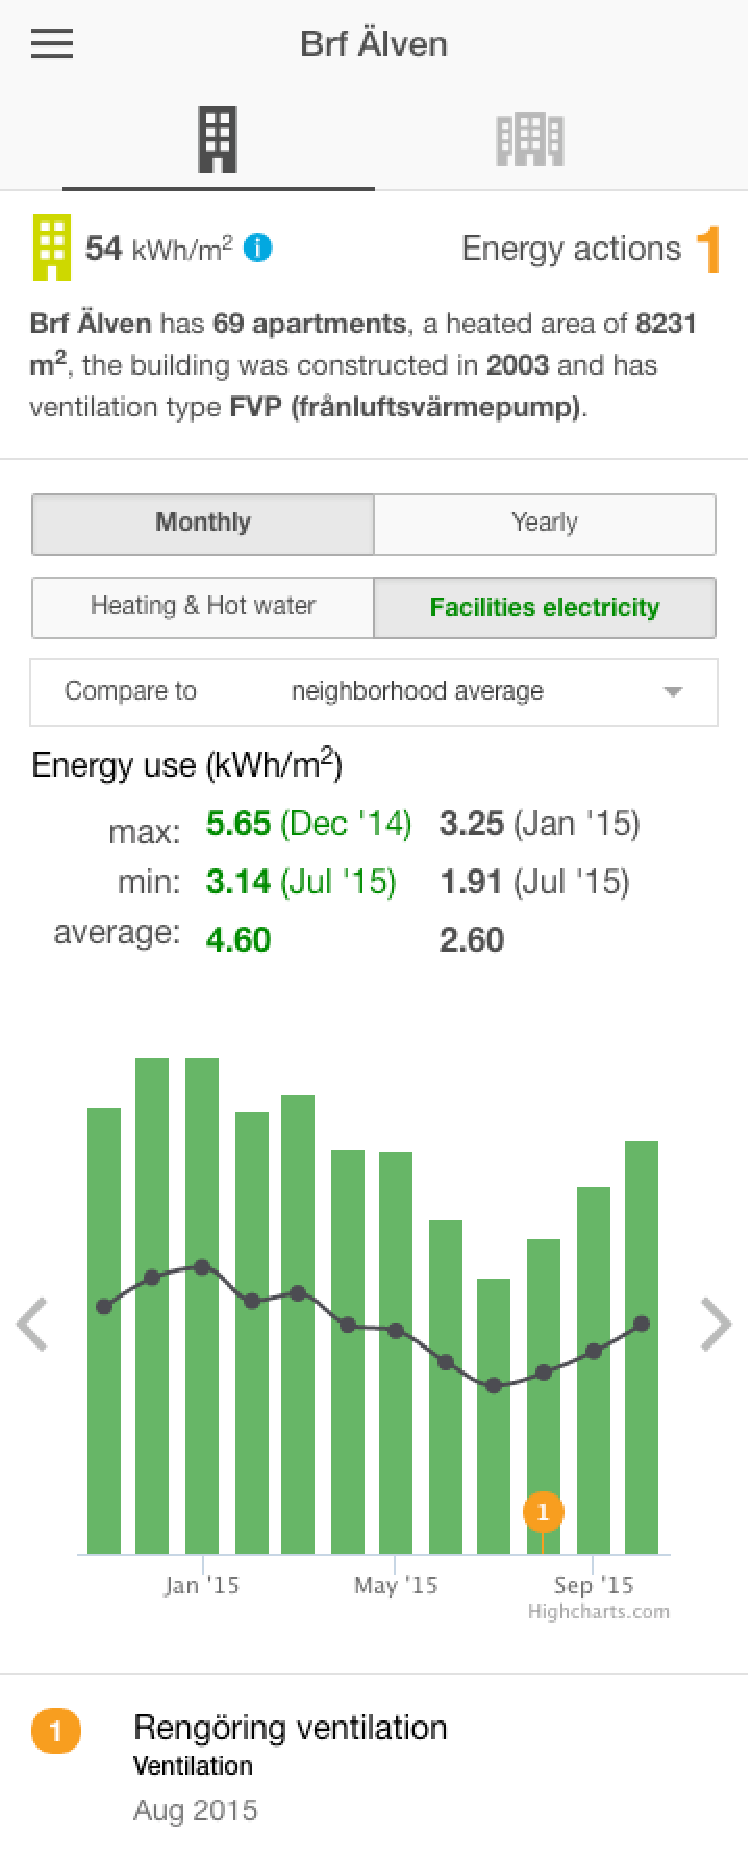
\includegraphics[width=0.7\linewidth]{img/brf.pdf}}
%\shadowimage[width=.25\linewidth]{img/action2.pdf}
%\shadowimage[width=.25\linewidth]{img/action1.pdf}
%\shadowimage[width=.25\linewidth]{img/action3.pdf}
%\caption{Action suggestion part of YouPower}
%\label{fig:action}
%\end{figure*}

%This part of YouPower aims to provide users easy access to practical and inexpensive suggestions (or tips) to (1) increase energy awareness, (2) inform energy know-how, and to (3) shape their long-term behaviors related to household energy consumption.
% 
%We collected about 50 suggestions (\url{https://goo.gl/R11QdZ}) from credible sources such as national and international energy agencies and associations. There are routine actions such as ``don't keep hot water flowing when you wash your dishes by hand'', regular actions such as ``defrost your fridge in $x$ days'', and one time actions such as ``install a programmable thermostat''.  
%Each action is accompanied with a short explanation that mainly focuses on intrinsic values to target long-term sustainable behaviors, the estimated impact and entailed effort (on a scale of 1 to 5), and the information about how many users are taking the action. 
%Users can choose to take a few actions at a time and are suggested with a new action when one is completed. 
%Some suggestions can be triggered by time, e.g., ``defrost your fridge in $x$ days.'' In such cases, the app reminds the users of the pending actions they are interested in. 
%A user has an ``action list'' that registers the user's actions. 
%
%When an action is completed, the user is awarded with points (displayed as \textit{Leaves}) associated to the effort and impact level of that action. 
%A user may also choose to abandon or reschedule an accepted action. 
%Upon action completion and cancellation, a user is asked to give feedback. 
%The user may ``like'' and ``share'' an action, rate the effort level of the action and give comments. 

%\begin{figure}
%\begin{center}
%	\begin{minipage}[t]{0.44\textwidth}
%	   \frame{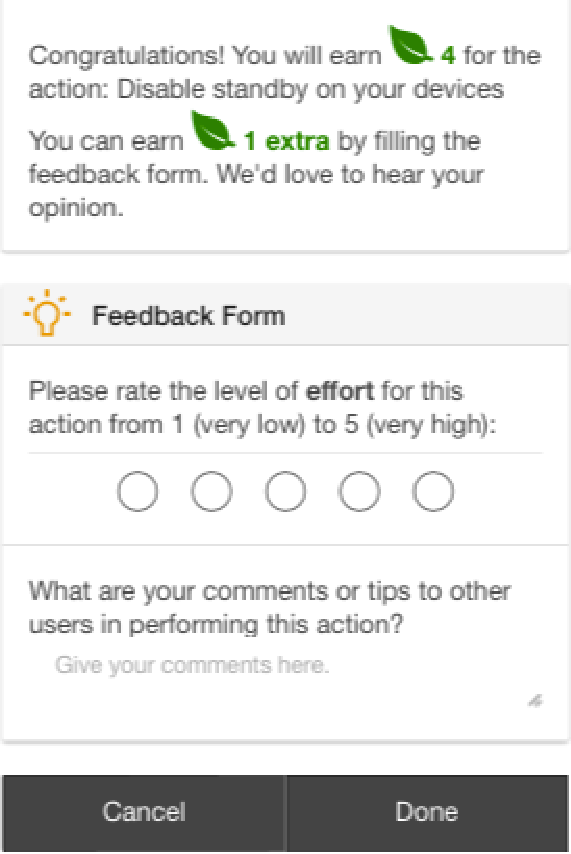
\includegraphics[width=\textwidth]{img/action_completed.pdf}}
%	    \caption{The feedback form when a user completes an action.}\label{fig:action_completed}
%	  \end{minipage}
%	  \hfill
%	\begin{minipage}[t]{0.44\textwidth}
%	   \frame{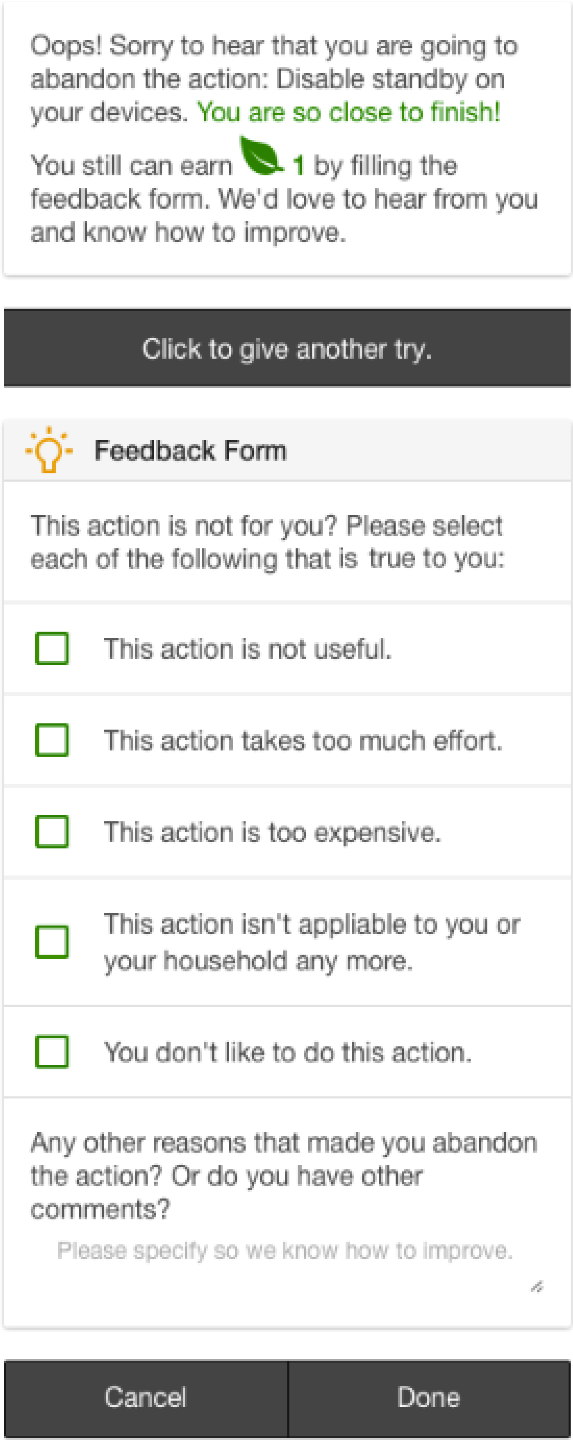
\includegraphics[width=\textwidth]{img/action_not_completed.pdf}}
%	   \caption{The feedback form when a user abandons an action.}\label{fig:action_not_completed}
%	  \end{minipage}
%\end{center}
%\end{figure} 



% 


%This application allows users to create and participate in community and personal energy challenges. It gives participants feedback on their performance during the challenge period and provides encouragement for participation using micro-actions. Users who performed well can share their success stories with other users. The application also allows for friends and group discussion. The community challenges can be incentivised by local investments (solar panels for the building), or through funding projects in developing countries (a school in Uganda). This application tries to motivate user engagement in energy community.

%\paragraph{Feedback on Achievements}
%In order to keep users motivated, we implement a set of achievements that are unlocked over time by using the app and performing the actions. For instance, users can get an achievement notification after they have performed a certain number of actions, accumulated a certain number of leaves individually or as part of some community, or after they have been using the app regularly for a certain period of time. Whenever a user unlocks an achievement in some category, s/he gets informed what is the next achievement in this category that s/he can reach. (E.g. ``Congrats! You completed your first $3$ actions! Your next goal is $5$ actions. Keep it up!'') Such achievements are based on the goal-setting \cite{Abrahamse2007265} and individual and collective feedback \cite{Abrahamse2013} approaches to behavioral changes in energy consumption.

%\paragraph{Personalization and Localization}
%A user has a personal profile and a household profile to customize the display name, preferred language (fot the whole app in English, Italian or Swedish), and to provide information about the household composition, home type and size, etc. The information is useful for personalized action suggestions and can be used for research purposes. A user can chose whether to link YouPower to the household's energy data. 
% In such cases, the app customizes its content to a user's test site: housing cooperatives content for the Swedish site and load-shifting content for the Italian site. They are discussed in the next two subsections. 


%\paragraph{Design Evaluation}
%The design was evaluated by peer reviews, a study with 24 participants 
%in an environmentally-oriented event in Helsinki (\url{https://oscedays.org/helsinki/}), 
%and a workshop with nine participants in the Italian test site. 
%% 
%In general, people liked the idea of receiving action suggestions. 
%They like to see the impact of their actions and asked for easy to perform actions. 
%The majority was interested in collaborative community actions, e.g., to save together and to donate for a common goal. Very few had interest in competition. 
% 
% Some people mentioned that the connection (or difference) between the \textit{Suggestions} and the \textit{Challenges} is hard to understand. Challenges were designed to express personal or community energy-goals, while suggestions are the means to achieve the goals. We later changed the name of this feature from \textit{Challenges} to \textit{Achievements}. 
% 
%Some people asked for the authority of the suggestions: it isn't clear where the tips come from. To what extent can they be trusted? Are they results of applied research? This is not marginal in a community of people who are quite familiar with energy-related issues. Having an explanation of how trustworthy these tips are would be very important. 
%%
%The meaning and value of the leaves are also another aspect that was questioned the most. 
%We thus decided to have an information page so that a number of such issues can be explained to the users. 
%In addition, users can send feedback to CIVIS through the app to keep the designers updated of users' concerns, questions, or other issues. 
% 
%Many expressed the opinion that monetary savings are only somewhat important to them. They were also skeptical about how much money they can actually save. They instead showed interest to learn about energy saving strategies as they are driven by more intrinsic motives.
%% 
%Some participants think that the others (in their neighborhood or city) do not put the same effort in energy conservation as themselves do. The YouPower approach to display other people's actions may have the potential to motivate people seeing the others' efforts.
%%
%Some suggested that for those who do not have or are not comfortable with smart-phones, the app should be made available through a browser. 






\section{\uppercase{Manuscript Preparation}}


\noindent {\bf Group 2.} Additionally, you may wish to copy and edit
the following 3 example files:
\begin{verbatim}
  - example.bib
  - example.tex
  - scitepress.eps
\end{verbatim}



\subsubsection{Tables}

\begin{table}[h]
\caption{This caption has more than one line so it has to be
justified.}\label{tab:example2} \centering
\begin{tabular}{|c|c|}
  \hline
  Example column 1 & Example column 2 \\
  \hline
  Example text 1 & Example text 2 \\
  \hline
\end{tabular}
\end{table}



%\begin{figure}[!h]
%  \vspace{-0.2cm}
%  \centering
%   {
\epsfig{file = SCITEPRESS.eps, width = 5.5cm}}
%  \caption{This caption has more than one line so it has to be justified.}
%  \label{fig:example2}
%  \vspace{-0.1cm}
%\end{figure}


\subsubsection{Equations}

Equations should be placed on a separate line, numbered and
centered.\\The numbers accorded to equations should appear in
consecutive order inside each section or within the contribution,
with the number enclosed in brackets and justified to the right,
starting with the number 1.

Example:

\begin{equation}\label{eq1}
    a=b+c
\end{equation}

\subsubsection{Program Code}\label{subsubsec:program_code}

Program listing or program commands in text should be set in
typewriter form such as Courier New.

Example of a Computer Program in Pascal:

\begin{small}
\begin{verbatim}
 Begin
     Writeln('Hello World!!');
 End.
\end{verbatim}
\end{small}


\section{\uppercase{Conclusions}}
\label{sec:conclusion}


\section*{\uppercase{Acknowledgements}}

\noindent This research is funded by the EU FP7 CIVIS project.
%It is also partly funded by the NWO project RobuSmart
%(Increasing the Robustness of Smart Grids through distributed
%energy generation: a complex network approach), grant number
%647.000.001. The authors would like to thank Jukka K. Nurminen from Aalto Univ. and Jan M�uller from KIT for their
%comments.


\bibliographystyle{apalike}
{\small
\bibliography{bib}}


%\section*{\uppercase{Appendix}}
%
%\noindent If any, the appendix should appear directly after the
%references without numbering, and not on a new page. To do so please use the following command:
%\textit{$\backslash$section*\{APPENDIX\}}

\vfill
\end{document}

